\documentclass{mefsdp}
 

\setauthors{Alp Gokcek, Erdal Sidal Dogan }
\settitle{TURKISH QUESTION GENERATION MODEL}
\setcourseno{I}
\setmonth{December}
\setyear{2020}
\setfaculty{Engineering}
\setdepartment{Computer Engineering}
\setchair{Prof. Muhittin Gokmen}
\setdate{04/12/2020}
\setadvisor{Asst. Prof. Seniz Demir}

\settitleTR{TÜRKÇE SORU OLUŞTURMA MODELİ}
\setmonthTR{Aralık}
\setfacultyTR{Mühendislik}
\setdepartmentTR{Bilgisayar Mühendisliği}
\setadvisorTR{Dr. Şeniz Demir}

\setfigurepath{../figures/}


\newacronym{dl}{DL}{Deep Learning}
\newacronym{qg}{QG}{Question Generation}
\newacronym{nlp}{NLP}{Natural Language Processing}

\usepackage{xcolor}
\usepackage{fancyvrb}
\usepackage{fvextra}

% redefine \VerbatimInput
\RecustomVerbatimCommand{\VerbatimInput}{VerbatimInput}%
{fontsize=\footnotesize,
	%
	frame=lines,  % top and bottom rule only
	framesep=2em, % separation between frame and text
	rulecolor=\color{black},
	%
	labelposition=topline,
	%
	commandchars=\|\(\), % escape character and argument delimiters for
	% commands within the verbatim
	commentchar=*        % comment character
}

\begin{document}
	
	\makestandards
	
	\begin{abstract}
		In the last decade, computers and software we use has gained humanitarian characteristics. We talk with them, create chatbots that answer the question of the user as a real assistant and many more. All of this features are invigorated by the Artificial Intelligence research which has showed significant improvements over the past decade.
		
		With the emergence of the \gls{dl} systems, other sub-fields of AI such as \gls{nlp}  made leaps in short amount of time as well. Today, results of the studies of these fields are ubiquitous. \newline \par
		
		Development of such applications require extensively large datasets for the training of \gls{dl} models. These applications are helping us in many ways. They enable us to solve our problems with less effort in shorter amount of time, reduce the work loads on humans etc. \newline \par
		
		Development such applications require extensively large datasets. Datasets are crucial for a \gls{dl} model to be trained. Capability and the reliability of these applications are highly dependent on the data they have been trained on. \newline \par
		
		In this project, we aim to develop a Question Generation Model in Turkish Language.
		
		Furthermore, for an application to be developed in any language, training dataset must contain the examples from that language as well. Sourcing such data in languages such as English, German, French etc. is not a hard task. However, labeled data in Turkish language is scarce, hence, development of smart applications such as question bots, personal assistants etc. in Turkish requires significantly more effort comparing to other languages.
		
		 
		
		
	
		\keywords{
			Automatic speech recognition, Natural Language Processing, Deep Learning, Sentiment Analysis, MOOC\footnote{Massive Open Online Courses}}
	\end{abstract}
	
		
	\begin{abstractTR}
		Bu projenin amacı Wikipedia gibi mevcut çevrimiçi kaynakları kullanarak Türkçe Soru Üretme Sistemi geliştirmektir. Soru Üretme Sistemleri, verilen metin girişinden çeşitli mantıksal sorular üretebilen sistemlerdir. Bu sistemler, sohbet robotları, otomatik değerlendirme sistemleri vb. birçok bilgisayar uygulamasında yaygın olarak kullanılmaktadır. Bu tip uygulamaların Türkçe destekli olarak geliştirilmesinde çok önemli bir yeri bulunan Türkçe veri seti örneği bulunmadığından,. Bununla birlikte, QG araştırması İngilizce gibi diğer dillerde çoktan kayda değer bir seviyeye ulaştı ve bu görev için mevcut veri kümeleri var. Örneğin, Stanford Üniversitesi tarafından SQuAD, bu görev için İngilizce olarak kullanılan iyi bilinen veri kümelerinden biridir. \newline \par
		Bu projede, orta büyüklükte ilk Türkçe Soru Üretme Veri Kümesini oluşturmayı hedefliyoruz. Bu adım, bu projede uygulayacağımız öğrenmeye dayalı çözümler geliştirmek için gereklidir. Çeşitli formlar (Kim-Ne-Ne Zaman vb.) Üretme soruları için farklı makine öğrenimi tabanlı teknikler uygulamayı ve toplayacağımız veri kümesindeki performanslarını değerlendirmeyi planlıyoruz.
		
		\anahtarkelimeler{Doğal Dil İşleme, Derin Öğrenme, Duygu Analizi}
	\end{abstractTR}
	
	\makelists

	\section{Introduction}
	Artificial Intelligence is one of the promising research fields of the computer science. Scientists and researchers are working for developing novel or more efficient ways to teach computers how to achieve humanly-kinds of tasks.\\
	
	Over time, developments in this area yield to whole new class of possibilities and of course problems that require brand new methodologies to be applied for reaching to the solution. With the emergence of Machine Learning, computers became to be able to parse data, learn from the data and apply their findings from it in a way that they are told to.\\
	
	In the recent years, researchers came up with a more niche way of handling Machine Learning (ML) tasks, creating a structure that imitates the Neurons in our brains. This new subclass of ML is named Deep Learning (DL). Compared to ML, it is capable of handling much more complex task due to its multi-layered structure.\\
	
	Developments in this area enabled researches from numerous fields to move their research a step further. Today, Deep Learning is ubiquitous in computer applications. It is utilized for Computer Vision, Natural Language Processing, Biotechnology and so on. In this project, methods and techniques that are results of the studies conducted in the research area of Natural Language Processing are used heavily along with various Machine Learning and Deep Learning models. Consequently, Turkish Question Generation is invigorated by the state-of-art Deep Learning and Language Models.\\
	
	Turkish Question Generation Model aims to generate natural language questions from a given content, such as paragraphs, where the questions can be answered solely by the content.   As the authors, we find this task worth tackling since there are not many examples of comprehensive studies on the topic and the outcomes of this project will empower development of more-capable-than-ever Question Answering Systems for Turkish Language. 
	\newpage
	
	\subsection{Motivation}
	
	As humans we are constantly learn, adapt to changes or make decisions on everyday basis. Even if we don’t realize, we usually are dependent on other humans and their knowledge and expertise even for most trivial things we do in our daily lives.\\
	
	For instance, a student feels in need for an instructor or others than can address his/her questions about a topic, an individual may be in a hurry to find out whether he/she can perform SWIFT transaction from his bank, or simply a person can ask about the weather forecast to the voice assistant on a smartphone. All of these examples are having a common point that they are all based on Question Answering (QA) Systems.\\
	
	As we have discussed, QA Systems are being getting more and more space in our lives and presents wide range of opportunities. With these systems, we are able to get answers to our question at no time, without any human interaction at all. This feature enables humans to reach to even the most isolated information in the context a matter of time upon request.\\
	
	Unfortunately, given that almost every human spoken language has specific set of rules, grammar and vocabulary, QA systems needs to be developed for each language separately. Development of such systems are not easiest thing to do, first of all, even if the developer(s) has all the competency in the technical skills required, there is a need for clear, labeled, reliable and excessively large dataset. The dataset must contain questions and possible answers to that question. Creating such dataset manually is almost unattainable, therefore there is a need for a system that can automate this process. Question Generation systems are perfect for meeting such need. Output of the QG system can be used as the dataset for development.\\
	
	On top of that, QG systems can be utilized in the education field also. Given a passage, instructor may want to create various questions for the class automatically without putting any effort. Same application can be used by a student for practicing the learnings from a section.

	
	\subsection{Broad impact}
	\subsubsection{Global Impact of the solution}
	Online courses are gaining getting more and more popular each and every year. While their high-quality content available on web, for those people who are not able to understand English or mainstream languages of a specific subject, it is harder to keep up with the recent developments in the area. Up to this point, MOOC platforms offer translation and subtitles for such users. The Question Generation systems, along with Question Answering systems might be used for the purposes of creating an artificial interactive environment between the instructor and the student. Consequently, helping the information to spread around the world.
	
	\subsubsection{Economic Impact of the solution}
	This project enables us to move faster to the point where we can automate almost every Question-Answer process where the data is assumed to be available to computer system, there is not an ambiguity amongst possible answers and the answers are static and clearly defined or quantitative.\\
	
	Initial assumption would be that such system would decrease the human dependency and reduce the number of jobs consequently. However, given that the same approach is applicable to almost every new technology/product emerges in the market, it is shown that they also create new opportunities. 
	
	
	\subsubsection{Environmental Impact of the solution}
	Since the project will be software based, no significant effect on environment will be observed. Of course, one can discuss that keeping the servers on, utilizing their resources to the maximum level continually will increase the total electricity consumption. 
	
	\subsubsection{Societal Impacts of the solution}
	This project has many social impacts, though not directly. With the solution we developed, strengthening the question-answering model carried out in connection with this project, we will aid to the process of knowledge acquisitions for the learners.
	
	
	\subsubsection{Legal Issues related to the project}
	Such as any system that is designed to present information to the user, Question Answering systems, which our project Question Generation system will yield to development of, requires the necessary information for answering the question. Under this circumstances, source of this information is critically important. Consent of the creator must be obtained before developing such system. \\
	
	Also, the system must not give inaccurate information to the user, since they may depend on the system on a critical task which fault can’t be tolerated at all.
	
	\section{Project Definition and Planning}
	Turkish Question Generation Model is a neural network-based model that is capable of generating questions from a given piece of text in Turkish Language. This project implements such model using \textit{Recurrent Neural Network (RNN)} and/or \textit{Convolutional Neural Network (CNN)}.
	
	\subsection{Project Definition}
	Main feature of the project will be accepting an input, create possible questions from that input while assigning probability scores to each of the generated questions. Questions are delivered in easily parsable file format such as JSON, XML, HTML, CSV, TSV etc.\\
	
	There is not a GUI is planned for the QG project, however it is going to be presented as CLI and \textit{Python Module}\footnotemark \footnotetext{An importable Python file that contains the functions for incorporating Turkish Question Generation for further research.} servers. for public use if allowed.
\\
	
	\begin{figure}[ht!]
		\centering
		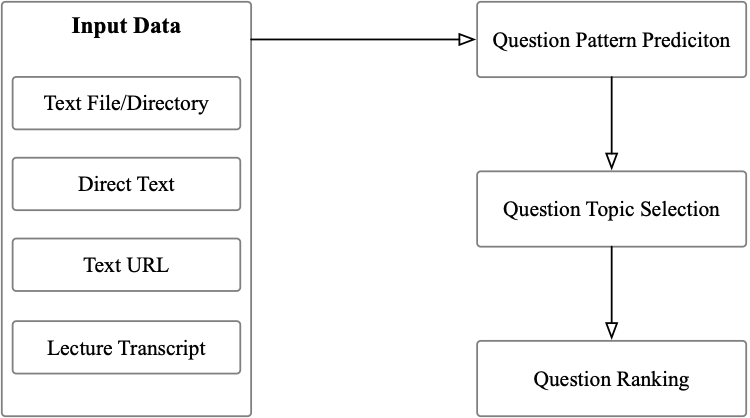
\includegraphics[scale=.8]{qg-system-schema}
		\caption{Question Generation system schema}
	\end{figure}

	\subsubsection{Dataset}
	There are lots of publicly available datasets for natural language processing tasks. However, for this project our main constraint was to build our system on top of a Turkish Dataset. Some other constraints we had was that the data must consist of correctly structured sentences in grammatical aspect, it must be labeled, come from a reliable source with the consent of the owner(s) and must be very large, given that larger dataset yields better models.
	
	\subsubsection{Programming Languages and Frameworks}
	This project is developed with \textit{Python 3}. It has chosen because it is relatively simple and allows us to focus on the project rather than computational concerns, it has a very large community for troubleshooting, which also decreases the chances of having issue about the language.\\
	
	Furthermore, Python is adapted by the AI researchers and there are numerous resources, frameworks and libraries that is developed for Python in which we utilize heavily. Framework we are going to be using is PyTorch. This framework recently developed and provides state-of-art parallel processing of tenors on GPU. Also, there are other libraries that are developed for scientific computing and has been used in this project such as pandas, NumPy etc.\\
	
	\subsection{Project Planning}
	\begin{table}[ht!]
		\caption{Project plan for 14 weeks}
		\centering
		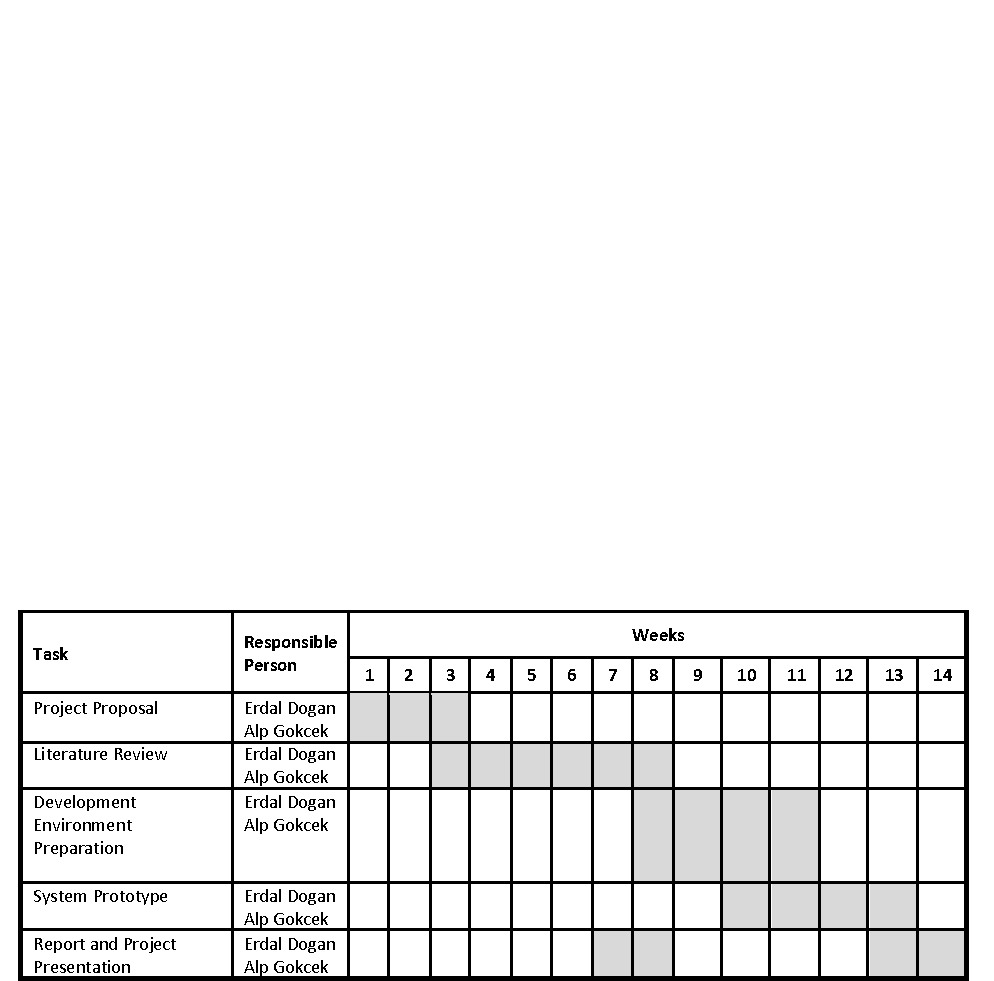
\includegraphics[scale=.8]{gantt}
	\end{table}
	\newpage
	\subsubsection{Aim of the project}
	Turkish Question Generation Model aims to create a Deep Learning model that given a paragraph, passage or an entity in Turkish, it presents the possible questions that can be answered solely by the given content to the system.
	
	\begin{figure}[ht!]
		\centering
		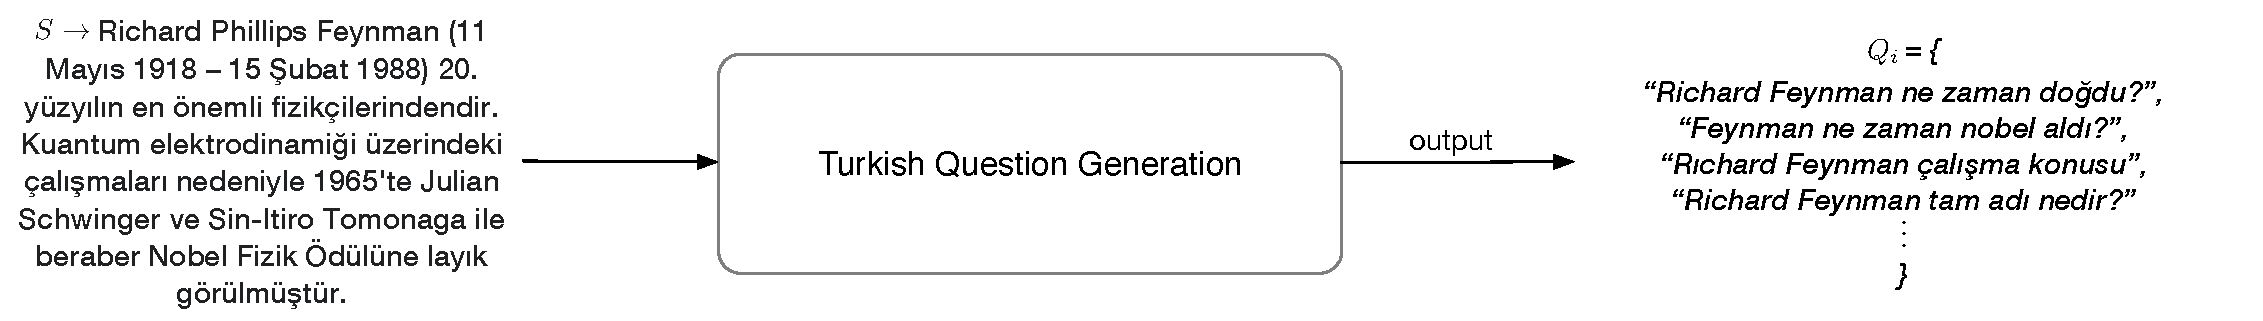
\includegraphics[scale=.37]{turkish_qg_system}
		\caption{Question Generation Model diagram}
	\end{figure}

	\subsubsection{Project Coverage}
	The project consists of sequential stages where the given input is passed over from one to other. These stages can be classified as the main content of the project. Initially, there will be a pre-processing stage for the data, this pre-process might be tweaking the string or simplifying the sentence. Then, BERT language model will be fine-tuned upon retrieving the input string.\\
	
	Project is based on software; outcome and the deliverables will consist of soft materials. Outcome of the project will be an executable file and/or importable Python module that can be used by other researchers.
	
	
	\subsubsection{Use Cases}
	% TO-DO
	Provide UML use case diagrams by specifying systems, actors, use cases and relationships.
	\newpage
	
	\subsubsection{Success Criteria}
	Outcomes of the project will be evaluated by couple of metrics. Given that the outputs will be natural language instances, existing methods and algorithms specifically designed for evaluation of generated natural language examples will be utilized. There are multiple algorithms and methods available, which consider different aspects of the outcome. Some of them are:
	\begin{itemize}
		\item BLEU
		\item ROUGE
		\item METEOR\\
	\end{itemize}
	
	Each of the enumerated methods are taking different aspects into account, while \textit{BLEU} score is calculated with best match length is prominent, \textit{ROGUE} is based on recall score. They all have their tradeoffs and neither of them is merely strong indicator of success.
	
	\subsubsection{Project time and resource estimation}
	The project is estimated to take 16 weeks for 2 undergraduate students that are novices to topic. While estimating, course load and other external factors are taken into account. Detailed timeline can be seen from Table 1 at the previous page. \\
	
	Assuming that each member spends 8 hours a week working on issues that are related to this project, it makes approximately 128 hours per person, 256 hours spent in total. Also, it has been mentioned that computing resources will be required for the project. If we use cloud computing provider’s (AWS for this particular example) rates for this estimation, we observe that hourly price is ~\$2 for a server that we need to run. Considering the fact that these are very intensive applications, it might be the cases that server will be up and making computations for long hours, 20 hours a week. This estimation sums up to \$600 in server running costs and 256 men hours. Notice that not any access to books, online courses or any other learning material has not been included.
	
	
	\subsubsection{Solution Strategies and Applicable Methods}
	For the project we decided to use off-the-shelf language models by fine-tuning them according to our data. Of course, we could’ve tried to achieve it without using such advanced models, however, in this case there would be risk of not being able to complete the project in time or a flawed model could have been produced.\\
	
	We had an option to use another main-stream language model such as ELECTRA or RASA. Given that BERT was adopted by the community, faster to train and documentation is provided is more comprehensive than other, we decided to use BERT model.
	
	
	\subsubsection{Risk Analysis}
	One of the major risks that may occur is that the model is giving questions that are not directly related to given inputs or contain grammatical/structural errors. There are not any risks.
	
	\subsubsection{Tools Needed}
	The project requires the development of Machine and Deep Learning Models from scratch. Due to wide selection of libraries for this purpose, community behind it and being the de-facto standard of the AI research and scientific development, it has been decided that \textit{Python Programming Language} will be used for development and implementation during this project.\\
	
	Specifically, for the model development, an up-to-date, state-of-art library named \textit{PyTorch} will be used extensively. Also, development of such models and processing large amounts of data requires computing resources. Therefore, servers that are configured with GPU optimization in mind will be required for faster development process.
	
	
	
	\section{Theoretical Background}
	\subsection{Literature Survey}
	In this section, a survey of the literature from multiple sources could be found.
	\subsubsection{Question Answering}
	Question Answering (QA) is problem of automatically presenting the answers of the question that is asked by users without any human interaction. In a QA model, it is expected that the system has access to the necessary information to answer the question.\\
	In order to develop such model, we need excessively large data that consists of Questions and their Answers, a duple that we will denote by <Q, A>. Unfortunately, labeling this kind of data manually or creating answers from scratch for an Artificial Intelligence based solution is not the most efficient way.
	They address these problems by;
	\begin{enumerate}
		\item Large scale high-quality dataset from Community-QA websites such as Yahoo, Quora etc. is obtained, since they provide large scale QA pairs generated by real users.
		\item Two ways of accomplishing such task is implemented and compared. One is a retrieval based method using Convolutional Neural Networks(CNN) and other is generation-based method using Recurrent Neural Network (RNN).
		\item Outcomes of the QG model is integrated with end-to-end QA task. It is evaluated on three state-of-art datasets, SQuAD, MS MARCO, and WikiQA. Results show that generated questions can improve QA quality on all these three datasets.
	\end{enumerate}
	
	\begin{figure}[ht!]
		\centering
		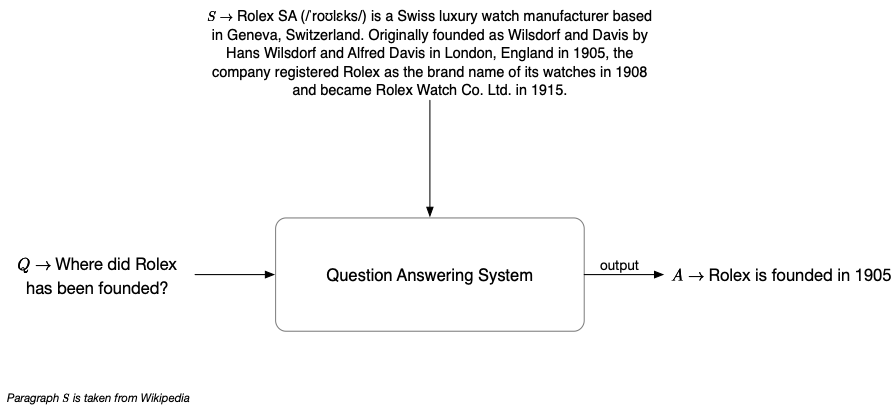
\includegraphics[scale=.8]{sample-qg}
		\caption{Sample Question Answering model}
	\end{figure}

	\subsubsection{Question Generation}
	In their paper, research engineers from Microsoft Research proposed a way of extracting question from a given piece of text. \cite{duan2017question} While they used NLP methodologies and Neural Networks for their paper, they didn’t include the semantics of words in their paper.\\
	
	QG Engine is consist of four components:
	\begin{enumerate}
		\item Question Pattern Mining
		\item Question Pattern Prediction
		\item Question Topic Selection
		\item Question Ranking
	\end{enumerate}
	\subsubsection{BERT Language Model}
	We have encountered a language model called BERT which is also known as Bidirectional Encoder Representation from Transformers developed by Google (Attention is all you need). It uses a machine learning model called Transformers. We have researched other language models and for the language translation problem, we have found two techniques which are LSTM and Transformers.\\
	
	First of all, we have found out that LSTMs are slow to train, words are passed sequentially and words are getting generated sequentially which can take significant time for the neural network to learn the language. And LSTMs are not truly bidirectional, they learn left to right and right to left separately and simply concatenate afterwards. This is where Transformers come. Transformers are faster because they can process words simultaneously and deeply bidirectional since they can learn in both directions. \\
	
	On the Figure \ref{transformer}, you can see the architecture of a transformer. It is formed by two components which are encoder and decoder.\\
	\begin{figure}[ht!]
		\centering
		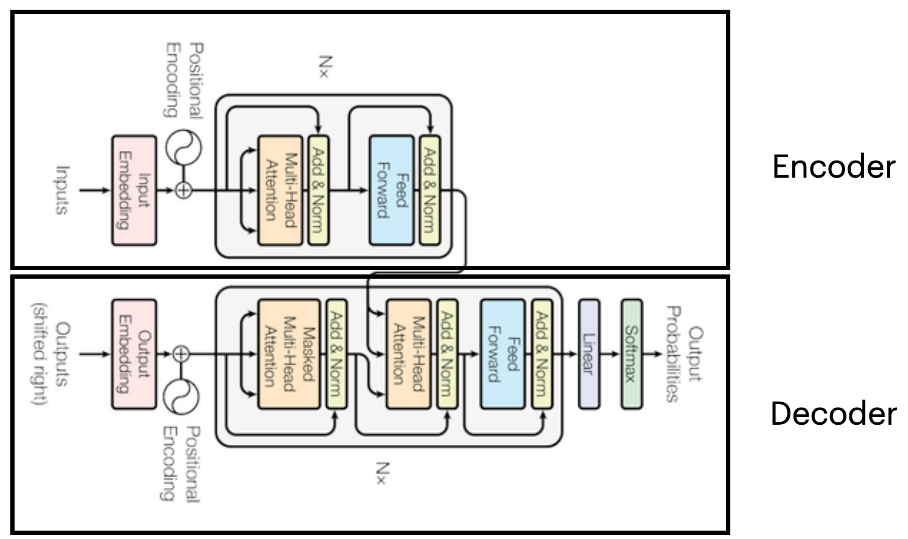
\includegraphics[scale=.8]{transformers}
		\caption{Architecture of a \textit{Transformer}\label{transformer}}
	\end{figure}

	As the BERT’s name suggests, if we put encoders on after another, we will obtain the BERT language model. The architecture of BERT language model could be found on figure \ref{bert-architecture}. It is the current state-of-the-art language model for NLP tasks. \cite{chan-fan-2019-recurrent}
	
	\begin{figure}[ht!]
		\centering
		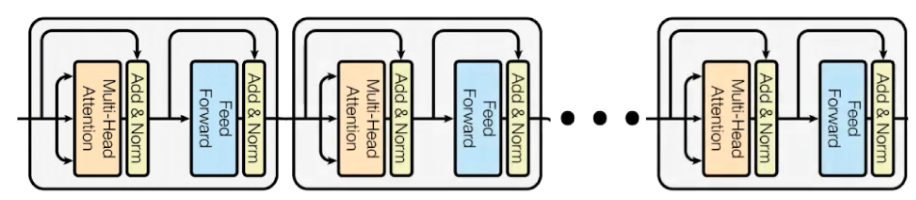
\includegraphics[scale=.8]{bert-model-architecture}
		\caption{BERT language model architecture\label{bert-architecture}}
	\end{figure}
	We have found a paper that uses this language model to solve our problem and they have made sequentially improved 3 models which are BERT-QG (BERT Question Generation), BERT-SQG (BERT Sequential Question Generation) and BERT-HLSQG (BERT Highlight Sequential Question Generation) models. QG is the simplest model that this paper introduces. It is the initial attempt to create a powerful Question Generation Model using BERT. As proposed by researchers, considering the previous decoded results significantly improve the quality of the model. However, in BERT-QG, token generation is performed without considering the previous states or decoded results. Due to this consideration, BERT-SQG is developed. BERT-SQG addressed the problem of ignoring the previous decodes in the BERT-QG model. However, researchers researched and concluded that BERT-SQG is not capable of producing quality questions in lengthy situations and if an answer phase appears multiple times it struggles to decide which one to decide. As a result, BERT-SQG is restructured and BERT-HLSQG, a model outperforming BERG-SQG is obtained.\\
	
	They have compared these models with the known to be best question generation models which were NQG-RC and PLQG. NQG-RC is a seq2seq question model based on bidirectional LSTMs. PLQG is a seq2seq network which is capable of handling long text input. This model is known to be the state-of-the-art models for QG tasks. As shown in table \ref{recurrent-comparison}, their models have outperformed the state-of-the-art models on every metric.\\
	\begin{table}[ht!]
		\caption{Performance comparison of Question Generation models on different datasets\label{recurrent-comparison}}
		\centering
		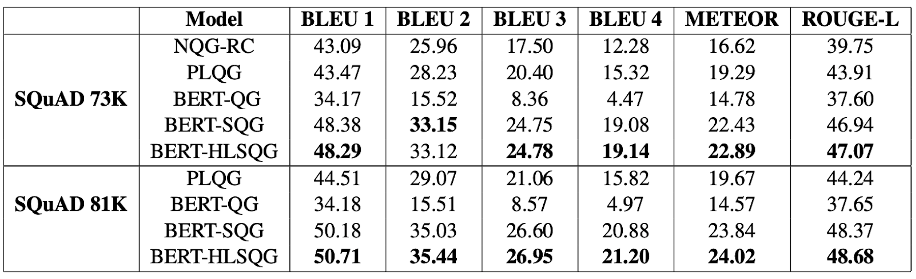
\includegraphics[scale=.7]{recurrent-comparison}
	\end{table}
	
	\subsection{Question Generation Model with BERT Language Model}
	As a result of this literature survey, we have decided to go with the BERT language model. BERT language model shows significant performance over various NLP tasks, such as classification, summarization, translation etc. It has a powerful architecture behind it which is transformers. We have searched a pre-trained Turkish model of BERT and we found a repository on GitHub for it. Starting from next week, we will start using this model as well.\\
	
	As the dataset, we have decided to go with Turkish Wikipedia dataset. There are several reasons behind it. Since the data of Wikipedia is close to textbook data, it should be beneficial to train our model with this dataset. And our advisor, Seniz Demir, had a Wikipedia Parser project. Thus, we will use Turkish Wikipedia dataset.
	
	
	
	\section{Analysis and Modeling}
	
	Aim of this project is to develop a Turkish Question Generation Model. Given a paragraph or a piece of text, our model creates the possible questions that can be answered with the information given in that paragraph. \newline \par
	
	However, development of such model requires an extensively large and labeled dataset that consist of paragraphs, corresponding question and answers to those questions. Unfortunately, such dataset is not available in Turkish Language. There are examples of it, but they neither contain large amounts of information nor we find the data reliable. \newline \par
	
	For the reasons described above, we decided to compose our own dataset. Our dataset consist of paragraphs from Turkish Wikipedia. By using the Person entities from the Turkish Wikipedia, we can create the question patterns for each attributes of a person. Later, these questions patterns are completed by substituting the person's name with the placeholders. At this step, we have our questions and the description paragraph of the person available to us.
	
	However, we must also confirm that the answer to the question is also found in the paragraph. For this reason, we use a fuzzy search algorithm in order to determine if the answer is in the paragraph or not. If it is, we add the questions to our dataset, if not we skip to next question. \newline \par
	
	Apart from the dataset, main goal of the project is to create the \gls{qg} model. Given that this model \gls{qg} model will be developed based on the dataset, first stage of this project has been dedicated to production of the dataset. 
	
	\subsection{System Factors}
	Since our work is based on the data acquired from Wikipedia and its manipulation, source data is highly effective on the outcome. While creating the dataset we always aim to create grammatically flawless questions while covering the variety of inputs that may come from the end-user
	
	\subsection{How System Works}
	Input data consists of ~53,000 person entities from Turkish Wikipedia. Occupations of each person and their attributes are also presented. For instance, for a 'Soldier', given attributes are: 'Rank', 'Wars', 'Nationality', 'Commanders' etc. Given that most of these attributes are also mentioned in the description paragraph of the corresponding person, when we create the questions that asks about these attributes, we will have the description paragraph and the questions together. 
	
	Initially, each question patterns for attributes are created manually containing a placeholder for the person's name. Later, by iterating over each person and substituting names for the their attributes we create an example of question. 
	
	When we iterate over every person, we accumulate a dataset which consist of paragraphs that describe the person, and questions about the attributes of the person which also is contained in the paragraph as well.  
	
	\subsubsection{Modelling}
	Explanation of system model.
	
	\subsubsection{System Architecture }
	Explanation of system architecture.
	
	\subsubsection{UML (Unified Modeling Language) Diagrams}
	
	\section{Design, implementation and testing}
	During the design phase of our project, we had two different components that have to be completed. These are:
	\begin{itemize}
		\item A Turkish question answering dataset that will be used to train the \gls{qg} model.
		\item A \gls{qg} model.
	\end{itemize}
	In this section, we will explain that what kind of design process we have followed during the design, implementation and testing of these two components separately.
	\subsection{Design}
	\subsubsection{Dataset}
	Before creating our dataset, we have researched if any of the datasets are suitable and sufficient. We have found one dataset that is suitable for our model. That dataset has around 2.2k questions, and the descriptive texts were about Turkish \& Islamic Science History, which is not completely suitable and sufficient. Hence, we have decided to create our dataset. During the design phase of the dataset, we have used 2 Wikipedia datasets. The first data was semi-cleaned scrapped Turkish Wikipedia data. Data we had has the short descriptions and the table contents. An example of the table content could be found in Figure \ref{wiki-table-content}. 
	\begin{figure}[h!]
		\centering
		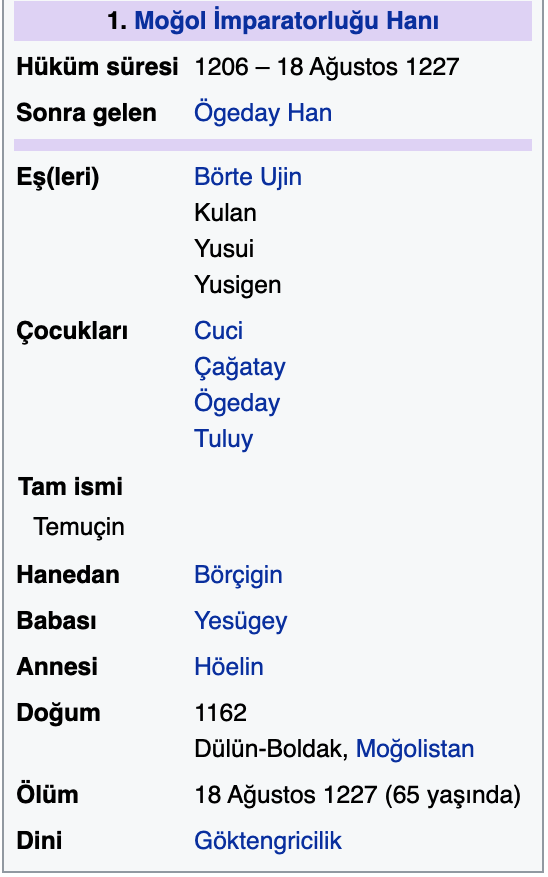
\includegraphics[scale=.3]{wiki-table-content}
		\caption{Sample Wikipedia table content\label{wiki-table-content}}
	\end{figure}

	However, this data was not sufficient for our dataset since most of the table contents' data does not appear on the short description. Thus, we had to use long descriptions for each of them. After that, we also matched the whole Wikipedia Turkish dump we found from Kaggle with our first data. This data had long descriptions of every document that is currently available on Wikipedia. During the matching phase, we have decided to match each document by their id's.\\
	
	After finishing the data part, we have started to analyze our data. We have grouped each person according to their occupation. After grouping, we have found out that we have twenty different occupations. Each occupation has its own table attributes. Our main goal is to generate question patterns according to their occupations and the most used 10 attributes for that specific occupation. Our analysis on the Wikipedia persons data could be found on Appendix A.\\
	
	Finally, we have started to generate the question patterns according to the occupation and the attributes. During this process, we have decided to the question pattern styling.\\
	
	\subsubsection{Question Generation Model}
	In the design process of Question Generation Model, we have followed the architecture of the \cite{chan-fan-2019-recurrent}. According to their architecture, we will use an sequential-to-sequential model. For the given paragraph $C=[c_1, c_2, ..., c_n]$, the answer phase $A=[a_1, a_2, ..., a_n]$ and the question $\hat{Q} = [\hat{q_1}, ..., \hat{q_i}]$, the input sequence $X_i$ will be shown as follows.
	\begin{equation}
		X_i =  ([CLS], C, [SEP], A, [SEP], \hat{q_1}, ..., \hat{q_i}, [MASK])\label{formula1}
	\end{equation}

	 There are 3 different tokens in that sequence. These can be summarized as follows:
	\begin{itemize}
		\item \textit{$[CLS]$}: Token shows the beginning of a sequence.
		\item \textit{$[SEP]$}: Token separates the answer from the context and the generated question.
		\item \textit{$[MASK]$}: Token shows the ending of a sequence.
	\end{itemize}

	After that, we take the final hidden state for the last token \textit{$[MASK]$} in the input sequence. We denote the final hidden vector of \textit{$[MASK]$} as $\textbf{h}[MASK] \in \textit{R}^{h}$. After that BERT model will be adapted by adding an affine layer $\textbf{W}_{SQG} \in \textit{R}^{h×|V|}$ to the output of the \textit{$[MASK]$} token. The label probabilities  $Pr(w|X_i) \in \textit{R}^{|V|}$ are computed by a soft-max function as follows. 
	\begin{equation}
		Pr(w|X_i) = softmax(\textbf{h}[MASK] * \textbf{W}_{SQG} + \textbf{b}_{SQG})
	\end{equation}
	\begin{equation}
		\hat{q_i} = argmax_{w}Pr(w|X_i)
	\end{equation}
	Later on, on each iteration, the newly generated token $\hat{q_i}$ will be appended into X and the generation process will be continued until \textit{$[SEP]$} is predicted. Thus, in the end, we will have our question.
	\subsection{Implementation}
	Similar to the design part, we have developed each component separately.
	\subsubsection{Dataset}
	
	created We have generated around 1700 question patterns by hand.
	\subsubsection{Question Generation Model}
	\subsection{Testing}
	Explanation of the testing of your system.
	
	\section{Results}
	
	
	\section{Conclusion}
	Briefly explain the problem you studied, the solution method you proposed and your experience in the implementation. Then, please proceed to subsections and explain the requirements in details. 
	
	\subsection{Life-Long Learning}
	Identify additional knowledge, skills, and attitudes that you needed to complete the project. In the context of the project, which tools and methods did you learn by yourself?  From which sources did you learn them? How difficult was for you to learn these topics by yourself? How did you manage to collect the relevant information? Answer all the questions.
	
	\subsection{Professional and ethical responsibilities of engineers}
	Define professional and ethical responsibilities you followed during your design process. What are the professional and ethical standards you used in the project? Is there an ethics code or code of conduct? Answer all the questions.
	
	\subsection{Contemporary Issues}
	Evaluate you project experience in terms of contemporary issues related to the problem that you studied. What kind of contemporary tools you have used throughout your project? Analyze the contemporary issues related to the future of the field that you work in this project. What will change in the products, services, or processes in the next ten, twenty, or fifty years, with emerging technologies such as 3D printers, big data analytics, nanotechnology, internet of things, quantum computing, biotechnology, artificial intelligence, cognitive science, and robotics?
	
	\subsection{Team Work}
	During your design project experience, describe the team work that you have participated. Give positions and majors of the people in the company that you worked with. Evaluate the composition, organization, and performance of your team. Describe how you shared the load in terms of the project tasks. 
	
	\begin{appendix}[A]
		\VerbatimInput[breaklines=true, label=attributes.txt\label{attributes}]{./attributes.txt}
	\end{appendix}

	\begin{appendix}[B]
		Your Appendix goes here
	\end{appendix}
	
	\begin{acknowledgments}
		Your acknowledgments goes here
	\end{acknowledgments}
	
	\bibliographystyle{IEEEtranN}
	\bibliography{../bibliography/references}
\end{document}